\chapter{Modello Relazionale}

\section{Relazione}
Una {relazione} è definita da uno {schema} e dalle {istanze} della relazione (dette anche {stato} della relazione)

\section{Attributo}
L'attributo di una relazione (attributo relazionale) è definito come una coppia $A_i:T_i$ dove $T_i$ è il tipo dell'attributo e $A_i$ è il nome dell'attributo.

\subsection{Tipologia}
Un tipo $T_i$ è caratterizzato da:
    \begin{itemize}
        \item{$T_i$: nome \textbf{identitificativo} del tipo}
        \item{$D_i$: \textbf{dominio} di valori}
        \item{Collezione di \textbf{operazioni} abilitate ad agire su $D_i$}
        \item{Operazioni di \textbf{confronto} su $D_i$}
    \end{itemize}
\textbf{Tipi standard}: \texttt{Integer}, \texttt{Real}, \texttt{String}, \texttt{Char}, \texttt{Date}, \texttt{Boolean}\\
\textbf{Tipi utente}: \text{tipo enumerativo}.

\subsection{Dominio}
Un tipo è sempre associato ad un dominio, ovvero a un insieme (potenziale infinito) di valori.\\\\
Possiamo immaginare una funzione
    \begin{equation}\begin{aligned}
        \text{dom}(A_i) = D_i
    \end{aligned}\end{equation}

\subsection{Valore nullo}
Per i casi in cui si riveli necessario inserire delle tuple con attributi mancanti in una relazione, è previsto un \textbf{valore nullo} (\texttt{NULL}), un vero e proprio valore, con la seguente proprietà generale:
    \begin{equation}\begin{aligned}
        \forall T_i, \quad \texttt{NULL} \in D_i
    \end{aligned}\end{equation}
Cioé, il valore \texttt{NULL} appartiene al dominio $D_i$ di qualsiasi tipo $T_i$.

\section{Schema di una relazione}
Lo \textbf{schema di una relazione} è un insieme di attributi, espressi con la seguente notazione:
    \begin{equation}\begin{aligned}
        \{  A_1:T_1, ..., A_n:T_n   \}\\
        R ( A_1:T_1, ..., A_n:T_n   )
    \end{aligned}\end{equation}
Spesso, per semplificare, si sottintende il tipo (che, però, deve sempre essere specificato nei DBMS):
    \begin{equation}\begin{aligned}
        \{  A_1:T_1, ..., A_n:T_n   \}
        \quad \rightarrow \quad
        \{  A_1, ..., A_n   \}\\
        R ( A_1:T_1, ..., A_n:T_n   )
        \quad \rightarrow \quad
        R ( A_1, ..., A_n)
    \end{aligned}\end{equation}  
Definiamo l'insieme di attributi $A$ come:
    \begin{equation}\begin{aligned}
        A: \{  A_1:T_1, ..., A_n:T_n   \}
    \end{aligned}\end{equation}
Possiamo utilizzare la seguente notazione per indicare lo schema $R$:
    \begin{equation}\begin{aligned}
       R(A)
    \end{aligned}\end{equation} 

\section{Grado di una relazione}
La \textbf{cardinalità} $|A|$, anche detta \textbf{grado} della relazione, di uno schema di relazione è data dal numero di attributi dello schema.\\\\
L'insieme di attributi di uno schema di relazione è sempre un insieme non vuoto. Ergo:
    \begin{equation}\begin{aligned}
        |A| \geq 1
    \end{aligned}\end{equation}

\section{Istanza di una relazione}
Dato uno schema:
    \begin{equation}\begin{aligned}
        A: \{   A_1:T_1, ..., A_n:T_n\}
    \end{aligned}\end{equation}
Per semplicità, supponiamo che l'insieme $A$ sia ordinato.\\\\
L'\textbf{istanza}, o \textbf{stato} $r$ di una relazione è definito come un insieme di tuple per cui vale la proprietà:
    \begin{equation}\begin{aligned}
        <v_1, ..., v_n>:\\
        \forall i \quad v_i \in \text{dom}(A_i)
    \end{aligned}\end{equation}

\section{Cardinalità di una relazione}
La \textbf{cardinalità} $|r|$ dell'istanza di una relazione $r$ è data dal numero di tuple appartenenti alla relazione $r$ ed è detta semplicente \textbf{cardinalità della relazione}.\\\\
Contrariamente alla relazione, l'istanza di una relazione può essere vuota:
    \begin{equation}\begin{aligned}
        |r| \geq 0
    \end{aligned}\end{equation}

\section{Notazioni ibride}
Per indicare le relazioni utilizziamo lettere maiuscole:
    \begin{equation}\begin{aligned}
        R \text{ oppure } PAZIENTI
    \end{aligned}\end{equation}
Per indicare l'istanza delle relazioni utilizziamo lettere minuscole:
    \begin{equation}\begin{aligned}
        r \text{ oppure } pazienti
    \end{aligned}\end{equation}
Specifichiamo lo schema anche per le istanze:
    \begin{itemize}
        \item{$r(A_1, ..., A_n)$ o $pazienti(COD, Cognome, Nome, Residenza, AnnoNascita)$}
        \item{$r(R)$ o $pazienti(PAZIENTI)$: poco usate.}
        \item{$r$ o $pazienti$: se lo schema è ben chiaro}
    \end{itemize}
Possiamo usare anche la notazione tabellare:
    \begin{figure}[h!]
        \centering
        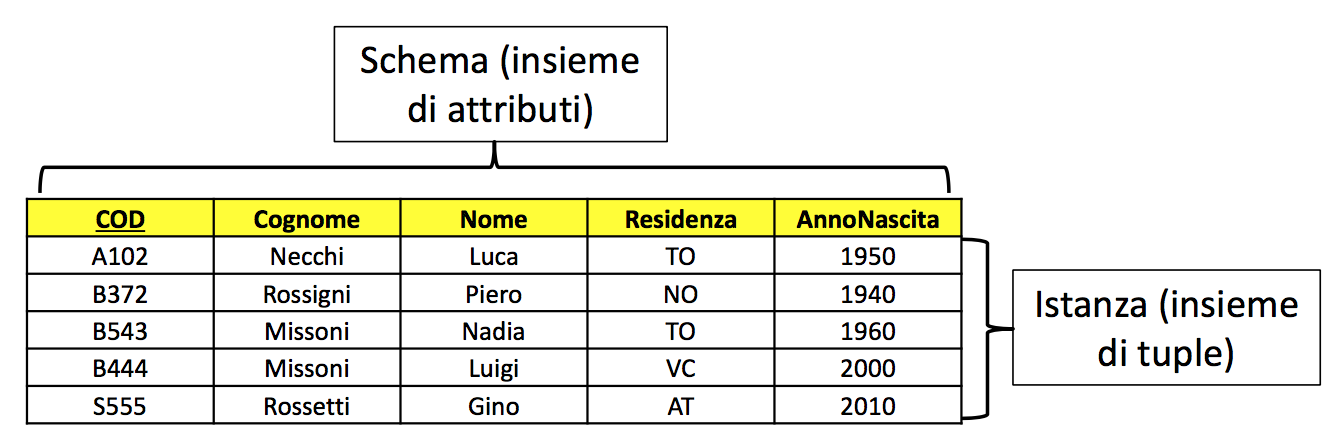
\includegraphics[scale = 0.5]{01/img01}
        \caption{Notazione tabellare}
    \end{figure}
Ciascuna relazione è definita da una coppia:
    \begin{equation}\begin{aligned}
        <R, r>
    \end{aligned}\end{equation}
dove $R$ è lo schema della relazione e $r$ è l'instanza della relazione.

\section{Tupla}
Data la relazione $r(A_1, ..., A_n)$,per indicare una singola \textbf{tupla} si usa la notazione
    \begin{equation}\begin{aligned}
        t = <v_1, ..., v_n>
    \end{aligned}\end{equation}
Poiché $t$ prende valori all'interno della relazione $R$:
    \begin{equation}\begin{aligned}
        t \in r (A_1, ..., A_n)
    \end{aligned}\end{equation}
    
\subsection{Valori di una tupla}
Per indicare il valore di una tupla $t$ in corrispondenza dell'attributo $A_i$ o di un insieme di attributi $A_i, ..., A_k$ si utilizzano le seguenti notazioni:
    \begin{equation}\begin{aligned}
        t[A_i] = v_i\\
        t.A_i = v_i\\
        t[A_i, ..., A_k] = <v_i, ..., v_k>\\
        t.(A_i, ..., A_k) = <v_i, ..., v_k>
    \end{aligned}\end{equation}
Per richiamare la tupla su tutti gli attributi si utilizzano le seguenti notazioni:
    \begin{equation}\begin{aligned}
        t, t[A], t.A
    \end{aligned}\end{equation}
Non essendo importante l'ordine degli attributi, la tupla non è altro che una \textbf{rappresentazione tabellare} che fa corrispondere a ogni attributo un valore del suo dominio:
    \begin{equation}\begin{aligned}
        t: A \rightarrow D
    \end{aligned}\end{equation}
    
\subsubsection{Esempio}
    \begin{center}\begin{tabular}{|c|c|} \hline
        \textbf{A} & \textbf{D}\\ \hline
        COD & A102 \\ \hline
        Cognome & Necchi \\ \hline
        Nome & Luca \\ \hline
        Residenza & TO \\ \hline
        AnnoNascita & 1950 \\ \hline
    \end{tabular}\end{center}
Possiamo adesso definire l'istanza $r$ di una relazione è dunque un insieme di funzioni
    \begin{equation}\begin{aligned}
        \{  t_1, ..., t_n   \}
    \end{aligned}\end{equation}
Ciascuna funzione $t_i$ definisce una particolare corrispondenza tra attributi e valori.\\
Le funzioni $t_i$ sono tutte distinte tra loro: ciò significa che in una relazione non può esistere una tupla identica a un'altra.\\\\
La tupla $t$ è \textbf{compatibile} con lo schema $A$ di una relazione se:
    \begin{itemize}
        \item{$t$ è una \textbf{funzione totale} su $A$.}
        \item{Ogni valore prodotto da $t$ appartiene a $D$.}
        \item{Vale il vincolo:
            \begin{equation}\begin{aligned}
                \forall A_i, \quad t.A_i \in \text{dom}(A_i)
            \end{aligned}\end{equation}}
    \end{itemize}

\section{Vincoli locali}
I \textbf{vincoli locali} sono caratterizzazioni dei valori possibili delle tuple in modo che tali valori rispettino (non siano in contrasto con) la realtà che vogliamo rappresentare.

\subsection{Vincolo locale di dominio}
Per ogni attributo abbiamo un insieme ben definito (anche infinito) di valori possibili.\\
Inoltre:
\begin{itemize}
    \item{Qualsiasi valore $v$ del dominio $D_i$ è atomico}
    \item{Un attributo il cui valore è una relazione non è atomico (solo alcuni DBMS, tra cui Oracle, lo permettono).}
\end{itemize}
Una relazione è \textbf{in prima forma normale} quando tutti gli attributi sono abbinati a domini di \textbf{valori atomici}.

\subsection{Vincolo sui valori nulli}
Un vincolo \texttt{NOT NULL} su un attributo $A_i$ è soddisfatto se, per ogni $t \in r$, il valore $t.A_i$ non è nullo.\\
Il funzionamento \textbf{pratico} è il seguente: al momento del caricamento dei dati in una tabella, il DBMS verifica che la tupla sia compatibile e che i valori degli attributi per cui è attivo il vincolo \texttt{NOT NULL} siano non nulli.

\subsection{Altri vincoli}
I DBMS forniscono la sintassi necessaria per la verifica dei seguenti vincoli:
    \begin{itemize}
        \item{\textbf{Restrizioni sui domini}: specificano i valori che non possono essere assunti da un particolare attributo.\\
            \textbf{ES:} una persona non può avere più di 120 anni, e non può essere nata nel futuro.\\
            \textbf{ES:} la temperatura corporea di un paziente non può superare i 42 gradi ed essere inferiore ai 34.}
        \item{\textbf{Confronti sui domini}: esprimono legami che devono essere rispettati da due o più attributi.\\
            \textbf{ES:} la data d'inizio ricovero dev'essere antecedente alla data di fine ricovero.}
    \end{itemize}

\subsection{Vincolo di identificazione}
Il vincolo di identificazione ci permette di identificare univocamente una tupla all'interno di uno schema, ed è espresso attraverso il vincolo di \textbf{chiave relazionale}.\\\\
Le chiavi relazionali possono essere composte da più valori, come nella tabella $RICOVERI$.\\\\
La nozione di vincolo di chiave relazionale è solitamente definita dal contesto applicativo (es. $COD$ dei $pazienti$ o $MATR$ dei medici).\\\\
Nella relazione di Codd gli elementi (tuple) dell'insieme (istnza) $r$ devono essere tutti distanti tra di loro.

\subsection{Definizione di superchiave}
Per poter definire in maniera formale il vincolo di chiave relazionale dobbiamo introdurre prima la nozione di superchiave.\\\\
Data una relazione $r(A)$, un sottoinsieme di attributi $sk \subseteq A$ è una \textbf{superchiave} 
    \begin{equation}\begin{aligned}
        \forall i,j \quad 
        (t_i[sk] = t_j[sk]) \rightarrow (t_i[A] = t_j[A])
    \end{aligned}\end{equation}
\textbf{ES:} nella tabella $PAZIENTI$, $(COD, Nome)$ è una superchiave.

\subsection{Chiave candidata}
$k \subseteq A$ è \textbf{chiave candidata} se:
    \begin{itemize}
        \item{$k$ è superchiave di $R$}
        \item{$k$ è superchiave \textbf{minimale} di $R$ (ogni sottoinsieme proprio di $k$ non deve soddisfare le condizione di superchiave).}
    \end{itemize}    
\textbf{ES:} $COD$ è superchiave, quindi $\{COD; Cognome\}$ non è chiave candidata.\\\\
Se $sk$ è una superchiave, allora $sk \subseteq w \subseteq A$ è una superchiave, quindi sono valide le seguenti \textbf{proprietà}:
    \begin{itemize}
        \item{$A$ è necessariamente una superchiave (per la definizione stessa di istanza, ogni tupla è distinta).}
        \item{$A$ è superchiave, quindi $A$ deve contenere sempre almneo una chiave candidata.}
    \end{itemize}

\subsection{Chiave principale}
La chiave principale $pk \subseteq A$ è una chiave scelta dal progettista tra tutte le possibili chiavi candidate.\\\\
Tutti gli attributi di una chiave principale devono rispettare in vincolo \texttt{NOT NULL}: una chiave candidata, invece, può ammettere valori nulli.

\section{Correttezza di una relazione}
Un'istanza di relazione $r(A)$ è corretta se ogni tupla $t \in r$ è compatibile con lo schema $A$ e sono soddisfatti tutti i vincoli locali (o intrarelazionali).

\section{Schema di una base dati}
Lo schema di una base dati è un insieme di schemi di relazione tutti con nome:
    \begin{equation}\begin{aligned}
        S = \{  R_1, ..., R_n   \}
    \end{aligned}\end{equation}
$S$ rispetta le seguenti proprietà:
    \begin{itemize}
        \item{I nomi devono essere tutti distinti}
        \item{Ad ogni schema si abbinano i rispettivi vincoli locali}
        \item{Ogni relazione $R_i$ esibisce una chiave principale}
    \end{itemize}

\section{Vincoli globali}
Così come è possibile definire dei vincoli locali (\textbf{intrarelazionali}) su ogni relazione $R$ è altresì possibile definire vincoli globali (\textbf{interrelazionali}) su uno schema di basi di dati $S$.

\subsection{Vincolo di integrità referenziale}
Consideriamo una relazione $R_h(\underline{PK}, ...)$ dove $PK$ è l'insieme di attributi della chiave principale, e una relazione $R_s(..., B, ...)$ dove $B$ è un insieme di attributi qualsiasi.\\\\
Esiste un \textbf{vincolo di integrità referenziale} degli attributi $B$ rispetto alla tavola $R_h$ se:
    \begin{equation}\begin{aligned}
        \forall t_i \\
        (t_i \in r (R_s))
        \quad \rightarrow \quad
        \exists t_j: [(t_j \in r(R_h)) \wedge (t_i[B] = t_j[PK])]
    \end{aligned}\end{equation}
Per poter creare il vincolo è necessario che i domini degli attributi in $PK$ siano compatibili con i domini degli attributi in $B$.    

\subsection{Vincoli globali generali}
I vincoli globali generali sono suggeriti dalle regole imposte dal sistema informativo e sono detti \textbf{regole di business}.\\\\
\textbf{ES:} in un sistema bancario con relazione $CONTOCORRENTE$ e relazione $MUTUO$, tutti i titolari di mutuo devono essere ten

\section{Base dati}
\subsection{Definizione di schema di una base dati}
La definizione dello schema $S$ di una base dati è completata dai vincoli globali.
\subsection{Stato di una base di dati}
Dato uno schema di base dati $S = \{    R_1, ..., R_n   \}$, lo \textbf{stato della base di dati} è definito come:
    \begin{equation}\begin{aligned}
        DB = \{ <R_1,r_1>,  ..., <R_n, r_n>   \}
    \end{aligned}\end{equation}
Dove ogni $r_i$ deve essere corretta e devono essere soddisfatti tutti i vincoli globali.

\section{Considerazione finale sul modello relazionale}
Il modello relazionale è un modello \textbf{orientato ai valori}.\\\\
Quando costruisco informazioni che coinvolgono tuple di relazioni diverse non posso che lavorare sui valori contenuti nelle tuple.\\
L'identificazione (chiave) di una relazione è basata sui valori presenti nella chiave.\\\\
In altri modelli (gerarchico, reticolare) le corrispondenze tra dati avvengono attraverso riferimenti (puntatori).
